\documentclass[12pt,a4paper, twosite]{article}
\usepackage[utf8]{inputenc}
\usepackage[T1]{fontenc}
\usepackage{graphicx}
\usepackage{grffile}
\usepackage{longtable}
\usepackage{wrapfig}
\usepackage{rotating}
\usepackage[normalem]{ulem}
\usepackage{amsmath}
\usepackage{textcomp}
\usepackage{amssymb}
\usepackage{capt-of}
\usepackage{hyperref}
\usepackage[left=2.00cm, right=2.50cm, top=2.50cm, bottom=2.00cm]{geometry}
\usepackage{fancyhdr}
\usepackage{datetime}
\usepackage{array}
\usepackage{tabularx}
\usepackage{booktabs}
\usepackage{array}
\usepackage{xcolor}
\usepackage{geometry}
\usepackage{colortbl}
\usepackage{helvet}
\usepackage{longtable}
\usepackage[spanish]{babel}
\renewcommand{\familydefault}{\sfdefault}
\geometry{margin=1in}
\fancyhead[RO,LE]{\thepage}
\fancyhead[LO]{\emph{\uppercase{\leftmark}}}
\fancyfoot{}
\renewcommand{\headrulewidth}{1.0pt}
\pagestyle{fancy}
\date{}
\title{Sistema de Extracción y Modelado de Datos con IA Embebida para la Optimización de Fertilización en Plantaciones de Tomate de Árbol}
\hypersetup{
pdfauthor={},
pdftitle={title},
pdfkeywords={},
pdfsubject={},
pdfcreator={Emacs 26.2 (Org mode 9.1.9)}, 
pdflang={English}}
\begin{document}

\begin{titlepage}
\begin{center}


\includegraphics[width=0.4\textwidth]{img/logo.png}\\[1cm]

{\huge\bfseries Master Test Plan}\\[2cm]

{\Large\textit{Sistema de Extracción y Modelado de Datos con IA Embebida para la Optimización de Fertilización en Plantaciones de Tomate de Árbol}}\\[2cm]

{\large Autor:\\
Leandro Quiroga.}\\[1cm]

{\large Maestría en Inteligencia Artificial Embebida\\
Universidad de Buenos Aires}\\[1cm]
{\large Marzo 2025}\\[1cm]
\vfill

\end{center}
\end{titlepage}

\section*{Historial de Cambios}
\begin{center}
\begin{tabular}{|c|c|c|c|c|}
\hline
\textbf{Versión} & \textbf{Fecha}  & \textbf{Descrición} & \textbf{Autor} & \textbf{Revisión} \\\hline
\hline
1.0 & \today & Versión original & Leandro Q. &  \\\hline\end{tabular}
\end{center}

\clearpage

\tableofcontents

\newpage

\section{Introducción}
\label{sec:introduccion}
Este documento describe el \textbf{Plan Maestro de Pruebas} del sistema de extracción y modelado de datos con IA embebida para la optimización de fertilización en plantaciones de tomate de árbol.
El sistema está constituido por dos placas de desarrollo: ESP32 y STM32, que funcionan como transmisor y receptor respectivamente. El dispositivo transmisor 
incorpora los sensores necesarios para la obtención de datos sobre nutrientes, condiciones del suelo y ubicación geográfica. Por su parte, el receptor se comunica con el transmisor a través de tecnología LoRa mediante una conexión punto a punto, permitiendo el almacenamiento de los datos recibidos y la ejecución de modelos predictivos que optimizarán el manejo del cultivo.
ver diagraam de flujo en el apendice \ref{sec:diagrama}

\section{Asignaciones}
\label{sec:asignaciones}

\subsection{Responsable}
El responsable de la elaboración de este documento es el Esp. Ing. Leandro Quiroga quien esta a cargo del proyecto

\subsection{Contratista}
La ejecución de las pruebas será realizada por el responsable del proyecto quien desarrollará y ejecutará las pruebas.

\subsection{Alcances}

\subsubsection{Dispositivo Transmisor (ESP32)}

\begin{enumerate}
  \item Adquisición de datos de sensores (N, P, K, EC, pH, temperatura, humedad).
  \item Visualización en pantalla TFT.
  \item Transmisión de datos vía LoRa.
\end{enumerate}

\subsubsection{Dispositivo Receptor (STM32)}
\begin{itemize}
  \item Recepción de datos y almacenamiento en microSD.
\end{itemize}

\subsubsection{Comunicación LoRa}
\begin{itemize}
  \item Fiabilidad (tasa de pérdida $<2\%$) y latencia ($<5$ segundos).
\end{itemize}

\subsubsection{Interfaz de Usuario:}
\begin{itemize}
  \item Operabilidad de pulsadores y claridad en la pantalla TFT.
\end{itemize}

\subsection{Precondiciones (externas)}
\begin{itemize}
  \item La documentación de las pruebas sera entregada para el 15 de Abril.
  \item El dispositivo estará disponible para test desde el 20 de Abril
  \item Los test deben finalizar el 30 de Abril.
\end{itemize}

\subsection{Precondiciones (internas)}
\begin{itemize}
  \item Las demoras del test deben ser reportadas al responsable del proyecto.
  \item El encargado del proyecto pondrá a disposición los recursos necesarios para la realización de las pruebas.
\end{itemize}

\section{Bases del test}

\begin{itemize}
  \item Especificación de requisitos de Software (ERS)
  \item Documento de Arquitectura: Diagramas de flujo funcional y especificaciones técnicas de hardware.
\end{itemize}

\section{Estrategia general del test}

\subsection{caracteristicas de calidad}
La siguiente tabla muestra las características de calidad seleccionadas para la estrategia general del test y su importancia relativa. Aquellas características que no se muestran en esta tabla no se consideran para este proyecto.

\begin{longtable}{|p{5cm}|p{7cm}|p{3cm}|}
  \hline
  \cellcolor[HTML]{4472C4}\textcolor{white}{\textbf{Característica}} & \cellcolor[HTML]{4472C4}\textcolor{white}{\textbf{Subcaracterística}} & \cellcolor[HTML]{4472C4}\textcolor{white}{\textbf{Importancia Relativa (\%)}} \\ \hline
  \textbf{Funcionalidad}  & Idoneidad (cumplimiento de requisitos)  & 35\% \\ \hline
  \textbf{Usabilidad}     & Operabilidad (interfaz intuitiva)       & 25\% \\ \hline
  \textbf{Precisión}      & Exactitud de datos y predicciones       & 20\% \\ \hline
  \textbf{Eficiencia}     & Tiempo de respuesta (<5 segundos)       & 15\% \\ \hline
  \textbf{Mantenibilidad} & Actualización de modelos y firmware    & 5\%  \\ \hline
  \caption{Características de Calidad} \label{tab:caracteristicas_calidad} \\
\end{longtable}


\begin{itemize}
  \item \textbf{Funcionalidad - Idoneidad (35\%)}: Esta es la característica más importante porque el sistema debe cumplir con todos los requisitos funcionales definidos. Si el dispositivo no adquiere los datos correctamente, no los almacena, no los transmite o no ejecuta los modelos predictivos como se especifica, el sistema no cumpliría su propósito principal. Es crucial que todas las funciones estén implementadas y funcionen según lo planeado.
  
  \item \textbf{Usabilidad - Operabilidad (25\%)}: Los usuarios finales son agricultores que pueden no tener mucha experiencia técnica. La interfaz debe ser intuitiva, con una pantalla TFT clara y pulsadores fáciles de usar. Si la operabilidad es baja, los usuarios podrían cometer errores o no utilizar el sistema eficientemente, lo que afectaría la adopción y efectividad del sistema.
  
  \item \textbf{Precisión - Exactitud (20\%)}: Los datos recopilados (niveles de nutrientes, pH, etc.) y las predicciones generadas deben ser precisos. Errores aquí podrían llevar a recomendaciones de fertilización incorrectas, perjudicando la producción. Además, la precisión en la geolocalización (GNSS) es vital para mapear correctamente las áreas de cultivo.
  
  \item \textbf{Eficiencia - Tiempo de respuesta (15\%)}: Aunque no es el factor más crítico, un tiempo de respuesta bajo (<5 segundos) asegura que los agricultores reciban retroalimentación rápida, especialmente en modo de predicción. Demoras excesivas podrían frustrar al usuario o afectar la toma de decisiones en tiempo real.
  
  \item \textbf{Mantenibilidad - Actualización (5\%)}: Aunque tiene el menor peso, es importante que el sistema permita actualizaciones de modelos de IA y firmware. Esto asegura que el sistema pueda adaptarse a nuevos datos o condiciones cambiantes en el campo, prolongando su vida útil y efectividad.
\end{itemize}

\subsection{Asignación de importancia relativa de las características de calidad en cada nivel de prueba}
Se indican a continuación, para cada nivel de prueba, las características de calidad y la importancia relativa de cada una de ellas.

\begin{longtable}{|p{3cm}|p{2cm}|p{2cm}|p{2cm}|p{2cm}|p{2cm}|}
  \hline
  \cellcolor[HTML]{4472C4}\textcolor{white}{\textbf{Nivel de Prueba}} & \cellcolor[HTML]{4472C4}\textcolor{white}{\textbf{Funcionalidad}} & \cellcolor[HTML]{4472C4}\textcolor{white}{\textbf{Usabilidad}} & \cellcolor[HTML]{4472C4}\textcolor{white}{\textbf{Precisión}} & \cellcolor[HTML]{4472C4}\textcolor{white}{\textbf{Eficiencia}} & \cellcolor[HTML]{4472C4}\textcolor{white}{\textbf{Mantenibilidad}} \\ \hline
  \textbf{Unitarias}          & 10\%  & –    & 40\%  & 20\%  & 30\%  \\ \hline
  \textbf{Integración SW}     & –     & –    & 30\%  & 50\%  & 20\%  \\ \hline
  \textbf{Integración HW/SW}  & 20\%  & 30\% & 30\%  & 20\%  & –     \\ \hline
  \textbf{Sistema}            & 40\%  & 30\% & 20\%  & 10\%  & –     \\ \hline
  \textbf{Aceptación}         & 50\%  & 40\% & 10\%  & –     & –     \\ \hline
  \textbf{Campo}              & 30\%  & –    & 50\%  & 20\%  & –     \\ \hline
  \caption{Asignación de Importancia por Nivel de Prueba} \label{tab:asignacion_importancia_prueba} \\
\end{longtable}

\subsection{Asignación de niveles de prueba a las características de calidad}
En la siguiente tabla se observa la relación entre los niveles de prueba y las características de calidad, donde "--" indica no aplicable, "+" indica importancia media y "++" indica alta importancia.

\begin{longtable}{|p{3cm}|p{2cm}|p{2cm}|p{2cm}|p{2cm}|p{2cm}|}
  \hline
  \cellcolor[HTML]{4472C4}\textcolor{white}{\textbf{}} & \cellcolor[HTML]{4472C4}\textcolor{white}{\textbf{Funcionalidad}} & \cellcolor[HTML]{4472C4}\textcolor{white}{\textbf{Usabilidad}} & \cellcolor[HTML]{4472C4}\textcolor{white}{\textbf{Precisión}} & \cellcolor[HTML]{4472C4}\textcolor{white}{\textbf{Eficiencia}} & \cellcolor[HTML]{4472C4}\textcolor{white}{\textbf{Mantenibilidad}} \\ \hline
  \textbf{Importancia Relativa} & 35\% & 25\% & 20\% & 15\% & 5\% \\ \hline
  \textbf{Unitarias}           & -    & –    & ++   & +    & +    \\ \hline
  \textbf{Integración SW}      & –    & –    & +    & ++   & +    \\ \hline
  \textbf{Integración HW/SW}   & +    & ++   & ++   & +    & –    \\ \hline
  \textbf{Sistema}             & ++   & +    & +    & -    & –    \\ \hline
  \textbf{Aceptación}          & ++   & ++   & -    & –    & –    \\ \hline
  \textbf{Campo}               & +    & –    & ++   & +    & –    \\ \hline
  \caption{Relación de Características y Componentes} \label{tab:relacion_componentes} \\
\end{longtable}

\section{Estrategia por nivel de prueba}

\subsection{Division del sistema en subsistemas}

El sistema se divide en subsistemas funcionales para facilitar la planificación y ejecución de pruebas. A continuación, se detallan los subsistemas definidos, agrupando componentes según su relevancia en el contexto de las pruebas:

\begin{longtable}{|p{6cm}|p{6cm}|p{2cm}|}
  \hline
  \cellcolor[HTML]{4472C4}\textcolor{white}{\textbf{Subsistema}} & \cellcolor[HTML]{4472C4}\textcolor{white}{\textbf{Descripción}} & \cellcolor[HTML]{4472C4}\textcolor{white}{\textbf{Importancia Relativa (\%)}} \\ \hline
  \textbf{Transmisor (ESP32)} & Sensores, almacenamiento, pantalla TFT y LoRa & 40\% \\ \hline
  \textbf{Receptor (STM32)} & Modelo predictivo, base de datos y comunicación & 30\% \\ \hline
  \textbf{Comunicación LoRa} & Transmisión punto a punto & 20\% \\ \hline
  \textbf{Interfaz de Usuario} & Pulsadores y pantalla TFT & 10\% \\ \hline
  \caption{Subsistemas y su Importancia Relativa} \label{tab:subsistemas_importancia} \\
\end{longtable}

\subsubsection*{Descripción detallada de los subsistemas}

\begin{itemize}
  \item \textbf{Subsistema A: Adquisición y procesamiento de datos}
  \begin{itemize}
    \item \textit{Componentes:} Sensores de suelo (N, P, K, EC, pH, temperatura, humedad), módulo GNSS.
    \item \textit{Funcionalidad:} Captura y procesamiento de datos en tiempo real. Valida la precisión de las lecturas y la integridad de los datos antes de su almacenamiento o transmisión.
  \end{itemize}
  
  \item \textbf{Subsistema B: Almacenamiento y visualización}
  \begin{itemize}
    \item \textit{Componentes:} Tarjeta microSD, pantalla TFT, pulsadores físicos.
    \item \textit{Funcionalidad:} Almacena datos en formato CSV y los muestra en la pantalla TFT según el modo seleccionado. Garantiza que la interfaz sea clara y responda a las interacciones del usuario.
  \end{itemize}
  
  \item \textbf{Subsistema C: Comunicación LoRa}
  \begin{itemize}
    \item \textit{Componentes:} Módulo LoRa en el transmisor (ESP32) y receptor (STM32).
    \item \textit{Funcionalidad:} Transmisión punto a punto de datos entre dispositivos. Valida la fiabilidad (<2\% de pérdida) y latencia (<5 segundos).
  \end{itemize}
  
  \item \textbf{Subsistema D: Modelado predictivo y almacenamiento}
  \begin{itemize}
    \item \textit{Componentes:} Modelo de IA embebido en el receptor (STM32), base de datos local/remota.
    \item \textit{Funcionalidad:} Ejecuta predicciones sobre fertilización, almacena resultados y permite actualizaciones del modelo. Asegura que las predicciones sean precisas (error <5\%) y no bloqueen otras tareas.
  \end{itemize}
  
  \item \textbf{Subsistema E: Gestión de energía y resiliencia}
  \begin{itemize}
    \item \textit{Componentes:} Circuito de alimentación, watchdog, mecanismos de reinicio.
    \item \textit{Funcionalidad:} Garantiza la estabilidad del sistema ante fallos (ej: cortes de energía, bloqueos).
  \end{itemize}
\end{itemize}

\subsection{Importancia relativa de los subsistemas }
La importancia se asigna según su impacto en la operación global del sistema:
\begin{longtable}{|p{6cm}|p{2.5cm}|p{6cm}|}
  \hline
  \cellcolor[HTML]{4472C4}\textcolor{white}{\textbf{Subsistema}} & \cellcolor[HTML]{4472C4}\textcolor{white}{\textbf{Importancia Relativa (\%)}} & \cellcolor[HTML]{4472C4}\textcolor{white}{\textbf{Justificación}} \\ \hline
  \textbf{A: Adquisición y procesamiento} & 35\% & Es la fuente primaria de datos. Errores aquí invalidan todo el flujo. \\ \hline
  \textbf{C: Comunicación LoRa} & 25\% & La transmisión fiable es clave para la sincronización transmisor-receptor. \\ \hline
  \textbf{D: Modelado predictivo} & 20\% & Las predicciones incorrectas afectan directamente la optimización del cultivo. \\ \hline
  \textbf{B: Almacenamiento y visualización} & 15\% & La interfaz intuitiva es crítica para la adopción por agricultores. \\ \hline
  \textbf{E: Gestión de energía} & 5\% & Secundario, pero necesario para operación continua. \\ \hline
  \caption{Importancia Relativa y Justificación de los Subsistemas} \label{tab:importancia_justificacion_subsistemas} \\
\end{longtable}

\subsection{Determinación de la importancia de test por combinaciones de subsistema y características de calidad}

\begin{longtable}{|p{5cm}|p{2cm}|p{2cm}|p{2cm}|p{2cm}|p{2cm}|}
  \hline
  \cellcolor[HTML]{4472C4}\textcolor{white}{\textbf{Subsistema}} & \cellcolor[HTML]{4472C4}\textcolor{white}{\textbf{Funcionalidad}} & \cellcolor[HTML]{4472C4}\textcolor{white}{\textbf{Usabilidad}} & \cellcolor[HTML]{4472C4}\textcolor{white}{\textbf{Precisión}} & \cellcolor[HTML]{4472C4}\textcolor{white}{\textbf{Eficiencia}} & \cellcolor[HTML]{4472C4}\textcolor{white}{\textbf{Mantenibilidad}} \\ \hline
  \textbf{A: Adquisición} & ++ & – & ++ & + & – \\ \hline
  \textbf{B: Almacenamiento} & + & ++ & + & – & – \\ \hline
  \textbf{C: Comunicación} & ++ & – & + & ++ & – \\ \hline
  \textbf{D: Modelado} & ++ & – & ++ & + & + \\ \hline
  \textbf{E: Energía} & + & – & – & + & – \\ \hline
  \caption{Relación de Subsistemas con Características de Calidad} \label{tab:subsistemas_caracteristicas_calidad} \\
\end{longtable}



\subsection{Determinación de las técnicas de test a ser utilizadas}

\begin{longtable}{|p{5cm}|p{5cm}|p{5cm}|}
  \hline
  \cellcolor[HTML]{4472C4}\textcolor{white}{\textbf{Subsistema}} & \cellcolor[HTML]{4472C4}\textcolor{white}{\textbf{Técnicas de Prueba}} & \cellcolor[HTML]{4472C4}\textcolor{white}{\textbf{Ejemplo de Caso}} \\ \hline
  \textbf{A: Adquisición} & 
  \begin{itemize}
    \item ECT (Pruebas de Comparación Elemental): Validar lecturas de sensores contra valores de referencia.
    \item CFT (Pruebas de Flujo de Control): Verificar secuencias de lectura/transmisión.
  \end{itemize}
  & Medir N, P, K en suelo con solución calibrada y comparar con valores del sistema. \\ \hline
  \textbf{B: Almacenamiento} & 
  \begin{itemize}
    \item STT (Pruebas de Transición de Estados): Alternar entre modos (recolección/predicción).
    \item Pruebas Heurísticas: Evaluar claridad de iconos y textos en TFT.
  \end{itemize}
  & Simular pulsaciones de botones para cambiar modos y validar respuestas en pantalla. \\ \hline
  \textbf{C: Comunicación} & 
  \begin{itemize}
    \item Pruebas de Estrés: Transmitir datos en condiciones de interferencia.
    \item Pruebas de Latencia: Medir tiempo entre envío y recepción.
  \end{itemize}
  & Enviar 1000 paquetes consecutivos y calcular tasa de pérdida. \\ \hline
  \textbf{D: Modelado} & 
  \begin{itemize}
    \item CTM (Método de Árbol de Clasificación): Validar predicciones con múltiples conjuntos de datos.
    \item Pruebas de Carga: Ejecutar modelo mientras se reciben datos.
  \end{itemize}
  & Comparar predicciones con resultados de laboratorio en 50 muestras de suelo. \\ \hline
  \textbf{E: Energía} & 
  \begin{itemize}
    \item Pruebas de Recuperación: Simular cortes de energía y validar reinicio.
  \end{itemize}
  & Desconectar alimentación durante operación y verificar recuperación automática. \\ \hline
  \caption{Técnicas de Prueba y Ejemplos de Caso por Subsistema} \label{tab:tecnicas_y_casos} \\
\end{longtable}
\newpage
\section{Apéndices}

\subsection{Diagrama de flujo del sistema}
l\label{sec:diagrama}
\begin{figure}[ht]
  \centering
  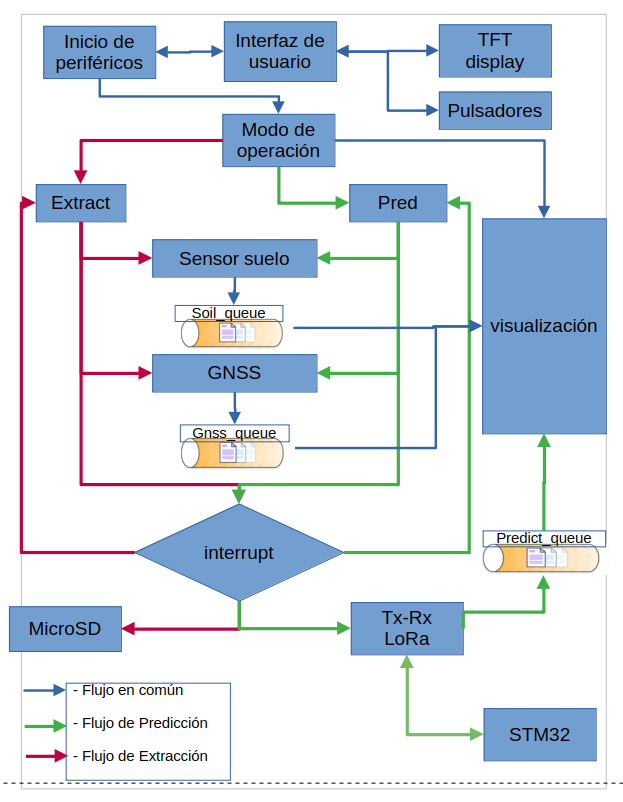
\includegraphics[width=0.8\textwidth]{img/system.png}
  \caption{Diagrama funcional del sistema}
  \label{fig:producer-consumer}
  \end{figure}

\end{document}